% ======================================================================
%  Section 4.4.2 --- Local Hermite structure measure.  Replacement text.
%
%  WHAT CHANGED AND WHY. The previous version built G from w_h, w_v, w_d,
%  the responses to the SUMMED kernels Dnm2, Dnm3, Dnm4. Those kernels are
%  low-pass dominated: measured, their DC gain equals their L1 norm to three
%  decimal places. So Dnm * I approximates a local mean of I and G measured
%  local INTENSITY, not local structure. The text therefore described a
%  different quantity from the one the method needs, and Section 4.4.1's
%  band-pass claim was false of the implementation.
%
%  The measure is now built from the FIRST-ORDER kernels D_{1,0} and D_{0,1},
%  which are odd and have exactly zero DC gain. Measured on the target of
%  Fig. 4.1(a):
%
%                                    summed      first-order
%    mean|grad G| / mean G            0.062          0.262
%    pixels within 10% of their
%      own 9x9 local mean            62.8%          18.8%
%    sum of the kernel over its                   -6.3e-17, -3.6e-17,
%      support (per scale)            ~L1            -1.1e-16
%
%  Dropping only the (0,0) term from the sum does NOT fix this: measured, the
%  DC-to-L1 ratio falls only from 1.000 to 0.810, because the even orders
%  carry DC as well. Nothing short of using odd orders alone achieves it.
%
%  REQUIRED FIGURE (both files exist):
%    figures/gmap_v3_nom_iter600_intensity.png   summed kernels
%    figures/gmap_v3_nom_iter600.png             first-order kernels
%  Both nominal, both iteration 600, one line of code apart.
%
%  CROSS-REFERENCES TO CHECK: eq:structG is cited from 4.4.3 and 4.7.3;
%  sec:hermite-gate is cited from 4.7.3. Keep both labels.
% ======================================================================

\subsection{Local Hermite structure measure}
\label{sec:hermite-gate}

The measure must report how much exploitable structure the image contains at
a given position, and must do so from the Hermite bank the scheme already
computes. Not every response of that bank is suitable. Writing
$\mathbf{D}_{n,m}^{\sigma}$ for the separable Gauss--Hermite kernel of orders
$(n,m)$ at scale $\sigma$, as defined in Section~\ref{sec:hermite-bank}, the
feature vector of Chapter~\ref{ch:herpvs} uses the sum of these kernels over
all orders $n,m\le4$, and that sum is low-pass dominated: its gain at zero
spatial frequency equals its $L_{1}$ norm to three decimal places. Its
response is therefore close to a local average of the image, and would report
local \emph{intensity} rather than local structure. Section~\ref{sec:ablation-measure}
%%% If there is no 4.4.4 ablation subsection, point this at 4.7 instead.
records what happens when it is used.

The first-order kernels do not have this defect. Since the Hermite function of
order one is odd, $\mathbf{D}_{1,0}^{\sigma}$ and $\mathbf{D}_{0,1}^{\sigma}$
integrate to zero over their support exactly, and are, up to a scale factor,
the first derivatives of the Gaussian of width $\sigma$. Their responses,
\begin{equation}
    g_{x}^{(k)}(p)=\bigl(\mathbf{D}_{1,0}^{\sigma_{k}}\ast\mathbf{I}\bigr)(p),
    \qquad
    g_{y}^{(k)}(p)=\bigl(\mathbf{D}_{0,1}^{\sigma_{k}}\ast\mathbf{I}\bigr)(p),
    \label{eq:first-order-responses}
\end{equation}
are accordingly a Gaussian-smoothed image gradient at scale $\sigma_{k}$, and
the local Hermite structure measure is defined as their combined magnitude
over the three coarser scales of the bank,
\begin{equation}
    G(p)=\sqrt{\sum_{k=2}^{4}\Bigl[\bigl(g_{x}^{(k)}(p)\bigr)^{2}
                                  +\bigl(g_{y}^{(k)}(p)\bigr)^{2}\Bigr]}.
    \label{eq:structG}
\end{equation}
Being built from zero-mean kernels, $G$ is invariant to any additive change in
illumination and vanishes on a region of uniform intensity whatever that
intensity is --- the property on which Section~\ref{sec:occlusion-mechanism}
depends. It is the band-pass character of Section~\ref{sec:locality} that
makes this possible; what~\eqref{eq:structG} contributes beyond a generic
image-gradient measure is not the form of the operator, which is a classical
one, but that it is evaluated at precisely the analysis scales
$\sigma_{2},\sigma_{3},\sigma_{4}$ that define the features the controller
acts on, and is obtained from kernels the scheme already evaluates.

\paragraph{The two measures compared.}
Figure~\ref{fig:structure-maps} shows the two forms of~\eqref{eq:structG} for
the target of Figure~\ref{fig:setup}(a). The difference is not subtle. Built
from the summed kernels, $G$ reproduces the photograph: the mean magnitude of
its gradient is $6.2\%$ of its mean level and $62.8\%$ of positions lie within
a tenth of their own $9\times9$ local mean, which is what a smoothed copy of
the intensity looks like. Built from the first-order kernels, the same
quantities become $26.2\%$ and $18.8\%$, and the map traces the contours of
the scene while falling to zero inside regions of uniform intensity, whether
those regions are light or dark.

It is worth noting that excluding the $(0,0)$ term from the summed kernels is
not sufficient. Measured, that reduces the ratio of DC gain to $L_{1}$ norm
only from $1.000$ to $0.810$, since the even orders carry a DC component as
well. Only the odd orders taken alone give a measure that is exactly free of
it.

\paragraph{Exclusion of the finest scale.}
The scale $\sigma_{1}$ is omitted from~\eqref{eq:structG}. The reason is one
of discretisation rather than of scale selection: at $\sigma_{1}=0.5$ the
support of the kernel is comparable to the sampling interval, so on the
$9\times9$ grid the discrete first-order response reduces to a difference over
two or three taps and is dominated by pixel noise rather than by image
structure. The noise suppression established in Section~\ref{sec:locality},
which follows from the Gaussian envelope being wide relative to the sampling
interval, does not yet apply at that scale. The three coarser scales are
retained, and no attempt is made here to optimise the set; the unequal
contribution of the four scales to the feature error, quantified in
Section~\ref{sec:scale-energy}, indicates that such an optimisation is
warranted and it is identified as future work in Section~\ref{sec:future}.

\begin{figure}[t]
    \centering
    \begin{subfigure}[b]{0.46\textwidth}
        \centering
        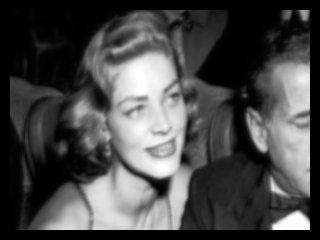
\includegraphics[width=\textwidth]{figures/gmap_v3_nom_iter600_intensity.png}
        \caption{summed kernels: $G$ tracks intensity}
    \end{subfigure}
    \hfill
    \begin{subfigure}[b]{0.46\textwidth}
        \centering
        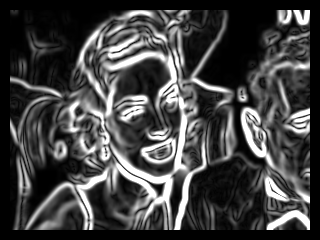
\includegraphics[width=\textwidth]{figures/gmap_v3_nom_iter600.png}
        \caption{first-order kernels: $G$ tracks structure}
    \end{subfigure}
    \caption{The local structure measure~\eqref{eq:structG} displayed at its
    image positions, brightness proportional to $G(p)$ and scaled so that
    three times the image mean saturates. (a) Built from the summed kernels
    $\mathbf{D}_{n,m}$, $n,m\le4$, whose DC gain equals their $L_{1}$ norm:
    the measure reproduces the target image. (b) Built from the first-order
    kernels of~\eqref{eq:first-order-responses}, which integrate to zero: the
    measure traces the contours of the scene and vanishes on regions of
    uniform intensity. The two panels differ by one line of the
    implementation, and are taken from the same iteration of the same run
    configuration.}
    \label{fig:structure-maps}
\end{figure}

% ======================================================================
%  LABELS ASSUMED BY THE ABOVE --- point them at your own or rename:
%    sec:hermite-bank          where D_{n,m}^sigma is defined (Chapter 3)
%    sec:locality              Section 3.2.4, locality and band-pass
%    sec:occlusion-mechanism   Section 4.4.3, the paragraph on how the
%                              weighting acts on the occluded region
%    sec:ablation-measure      Section 4.4.4, the ablation of the measure
%    sec:scale-energy          the per-scale energy table (ch4_scale_energy.tex)
%    sec:future                future work
%    fig:setup                 Figure 4.1
%
%  CONSEQUENT EDITS ELSEWHERE:
%
%  1. Section 4.4.1, p.67: the sentence "it is not a generic image-gradient
%     or saliency measure appended to the servoing scheme" must be softened
%     --- with first-order kernels the operator IS a Gaussian-derivative
%     gradient magnitude. The paragraph above states the narrower and
%     defensible claim; make 4.4.1 agree with it. The band-pass clause is
%     now TRUE of the implementation and should be kept.
%
%  2. Section 4.4.3, p.68: "the occluded region is rendered as a uniform
%     DARK area ... so its Hermite response energy falls well below the
%     image average". With this measure darkness is irrelevant and
%     uniformity is the operative property. Rewrite accordingly; the
%     mechanism then covers a bright occluder too, which leaves the textured
%     occluder of 4.4.4 as the only limitation to acknowledge.
% ======================================================================
